% Report and scan illustrations feed a shared model, followed by a task timeline.
\begingroup
\linespread{1}\selectfont
\definecolor{modelteal}{HTML}{24777B}
\definecolor{modelink}{HTML}{37474F}
\begin{tikzpicture}[
  font=\thesisfigurefont,
  box/.style={draw=modelink!70,rounded corners=2pt,line width=.65pt,align=center,inner sep=0pt},
  flow/.style={-{Latex[length=2mm]},draw=modelink,line width=.75pt,shorten <=1pt,shorten >=1pt},
  labeltext/.style={align=center,inner sep=0pt},
  task/.style={box,minimum width=3.75cm,minimum height=2.65cm,fill=black!1}
]
% Editable report sheets: visual placeholders only, without patient information.
\begin{scope}[shift={(1.05,-.05)}]
  \draw[draw=modelink!35,fill=black!3,rounded corners=1pt] (.14,.08) rectangle (1.69,1.63);
  \draw[draw=modelink!45,fill=white,rounded corners=1pt] (.07,.04) rectangle (1.62,1.59);
  \path[draw=modelink,line width=.7pt,fill=white] (0,0) -- (1.55,0) -- (1.55,1.24) -- (1.25,1.55) -- (0,1.55) -- cycle;
  \draw[draw=modelink,line width=.6pt] (1.25,1.55) -- (1.25,1.24) -- (1.55,1.24);
  \draw[draw=modelteal,line width=1.4pt] (.21,1.23) -- (.51,1.23) (.36,1.08) -- (.36,1.38);
  \draw[draw=modelink!70,line width=.7pt] (.7,1.28) -- (1.06,1.28) (.7,1.12) -- (1.12,1.12);
  \draw[draw=modelink!45,line width=.55pt] (.22,.87) -- (1.29,.87) (.22,.65) -- (1.29,.65) (.22,.43) -- (1.03,.43);
  \draw[draw=modelteal!60,line width=.55pt] (.22,.2) -- (.76,.2);
\end{scope}
\node[labeltext,anchor=west,font=\thesisfigurefont\bfseries] at (2.95,.98) {医学文本};
\node[labeltext,anchor=west,text=black!65] at (2.95,.45) {报告\enspace /\enspace 病史};
\node[inner sep=0pt] at (8.65,.7) {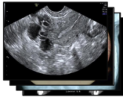
\includegraphics[height=1.5cm]{ch07/assets/example-000.png}};
\node[labeltext,anchor=west,font=\thesisfigurefont\bfseries] at (10.0,.98) {医学影像};
\node[labeltext,anchor=west,text=black!65] at (10.0,.45) {持续到达的数据};
\node[box,minimum width=2.8cm,minimum height=.6cm,fill=white] (textenc) at (3.025,-.95) {文本编码器};
\node[box,minimum width=2.8cm,minimum height=.6cm,fill=white] (imageenc) at (10.075,-.95) {图像编码器};
\draw[flow] (3.025,-.12) -- (textenc.north);
\draw[flow] (10.075,-.12) -- (imageenc.north);
\node[box,draw=modelteal,line width=1pt,fill=modelteal!5,minimum width=13.1cm,minimum height=1.55cm] (model) at (6.55,-2.48) {};
\node[labeltext,text=modelteal,font=\thesisfigurefont\bfseries] at (6.55,-2.02) {医学多模态基础模型};
\node[labeltext] at (6.55,-2.5) {影像\quad 文本\quad 结构\quad 知识};
\node[labeltext,text=black!65] at (6.55,-2.96) {跨模态融合\enspace /\enspace 共享表征\enspace /\enspace 版本记录};
\draw[flow] (textenc.south) -- (model.north -| textenc.south);
\draw[flow] (imageenc.south) -- (model.north -| imageenc.south);
\node[task] (task1) at (1.875,-5.48) {};
\node[task] (task2) at (6.55,-5.48) {};
\node[task] (task3) at (11.225,-5.48) {};
\node[labeltext,font=\thesisfigurefont\bfseries] at (1.875,-4.65) {任务一\\胸部 X 线诊断};
\node[labeltext,font=\thesisfigurefont\bfseries] at (6.55,-4.65) {任务二\\消化内镜识别};
\node[labeltext,font=\thesisfigurefont\bfseries] at (11.225,-4.65) {任务三\\皮肤镜分类};
\node[inner sep=0pt] at (1.875,-5.95) {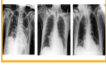
\includegraphics[height=1.35cm]{ch07/assets/example-001.png}};
\node[inner sep=0pt] at (6.55,-5.95) {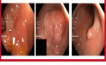
\includegraphics[height=1.35cm]{ch07/assets/example-002.png}};
\node[inner sep=0pt] at (11.225,-5.95) {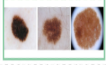
\includegraphics[height=1.35cm]{ch07/assets/example-003.png}};
\draw[flow] (model.south -| task1.north) -- (task1.north);
\draw[flow] (task1.east) -- (task2.west);
\draw[flow] (task2.east) -- (task3.west);
\node[labeltext,text=black!65] at (8.45,-3.72) {新模态、新任务、新中心与新知识};
\draw[flow,dashed,draw=modelteal!70] (3.75,-4.02) -- (13.1,-4.02);
\node[labeltext,text=black!65] at (6.55,-7.18) {顺序适配\quad $\longrightarrow$\quad 阶段评价};
\draw[draw=black!20,line width=.55pt] (0,-7.59) -- (13.1,-7.59);
\node[labeltext] at (6.55,-8.04)
  {\textbf{稳定性}\enspace 既有能力保持\qquad $\longleftrightarrow$\qquad \textbf{可塑性}\enspace 新增信息吸收};
\end{tikzpicture}
\endgroup
